\documentclass[a5paper,12pt]{article}
\usepackage{../../style}


\newcommand{\montitre}{Logique }


\begin{document}

\fiche{Histoire}
\titre{Logos} (grec) : le langage, le raisonnement\\

\titre{Définitions} : \begin{itemize}
	\item Etude du discours rationnel
	\item Etude de la raison dans le langage
	\item Science des conditions de vérité (d'une formule / d'un raisonnement)
\end{itemize}

\titre{Logique classique} : Socrate, Platon, Aristote jusqu'au début du $XIX^{eme}$ siècle. Analyse de la grammaire, prédominence de la logique aristotélicienne. \\

\titre{Logique moderne} : Symbolique et axiomatique. Mathématisée et algébrisée, elle repose sur un système hypothético-déductif et sur un système de réécriture. \\

\titre{Personnages importants} : Aristote, De Morgan, Boole, Gentzen, Russel\\

\titre{Méthodes} : L'étude des conditions de vérité d'une formule ou d'un raisonnement peut se faire par des méthodes \titre{sémantiques} ou \titre{syntaxiques}.


\fiche{Types de logique}
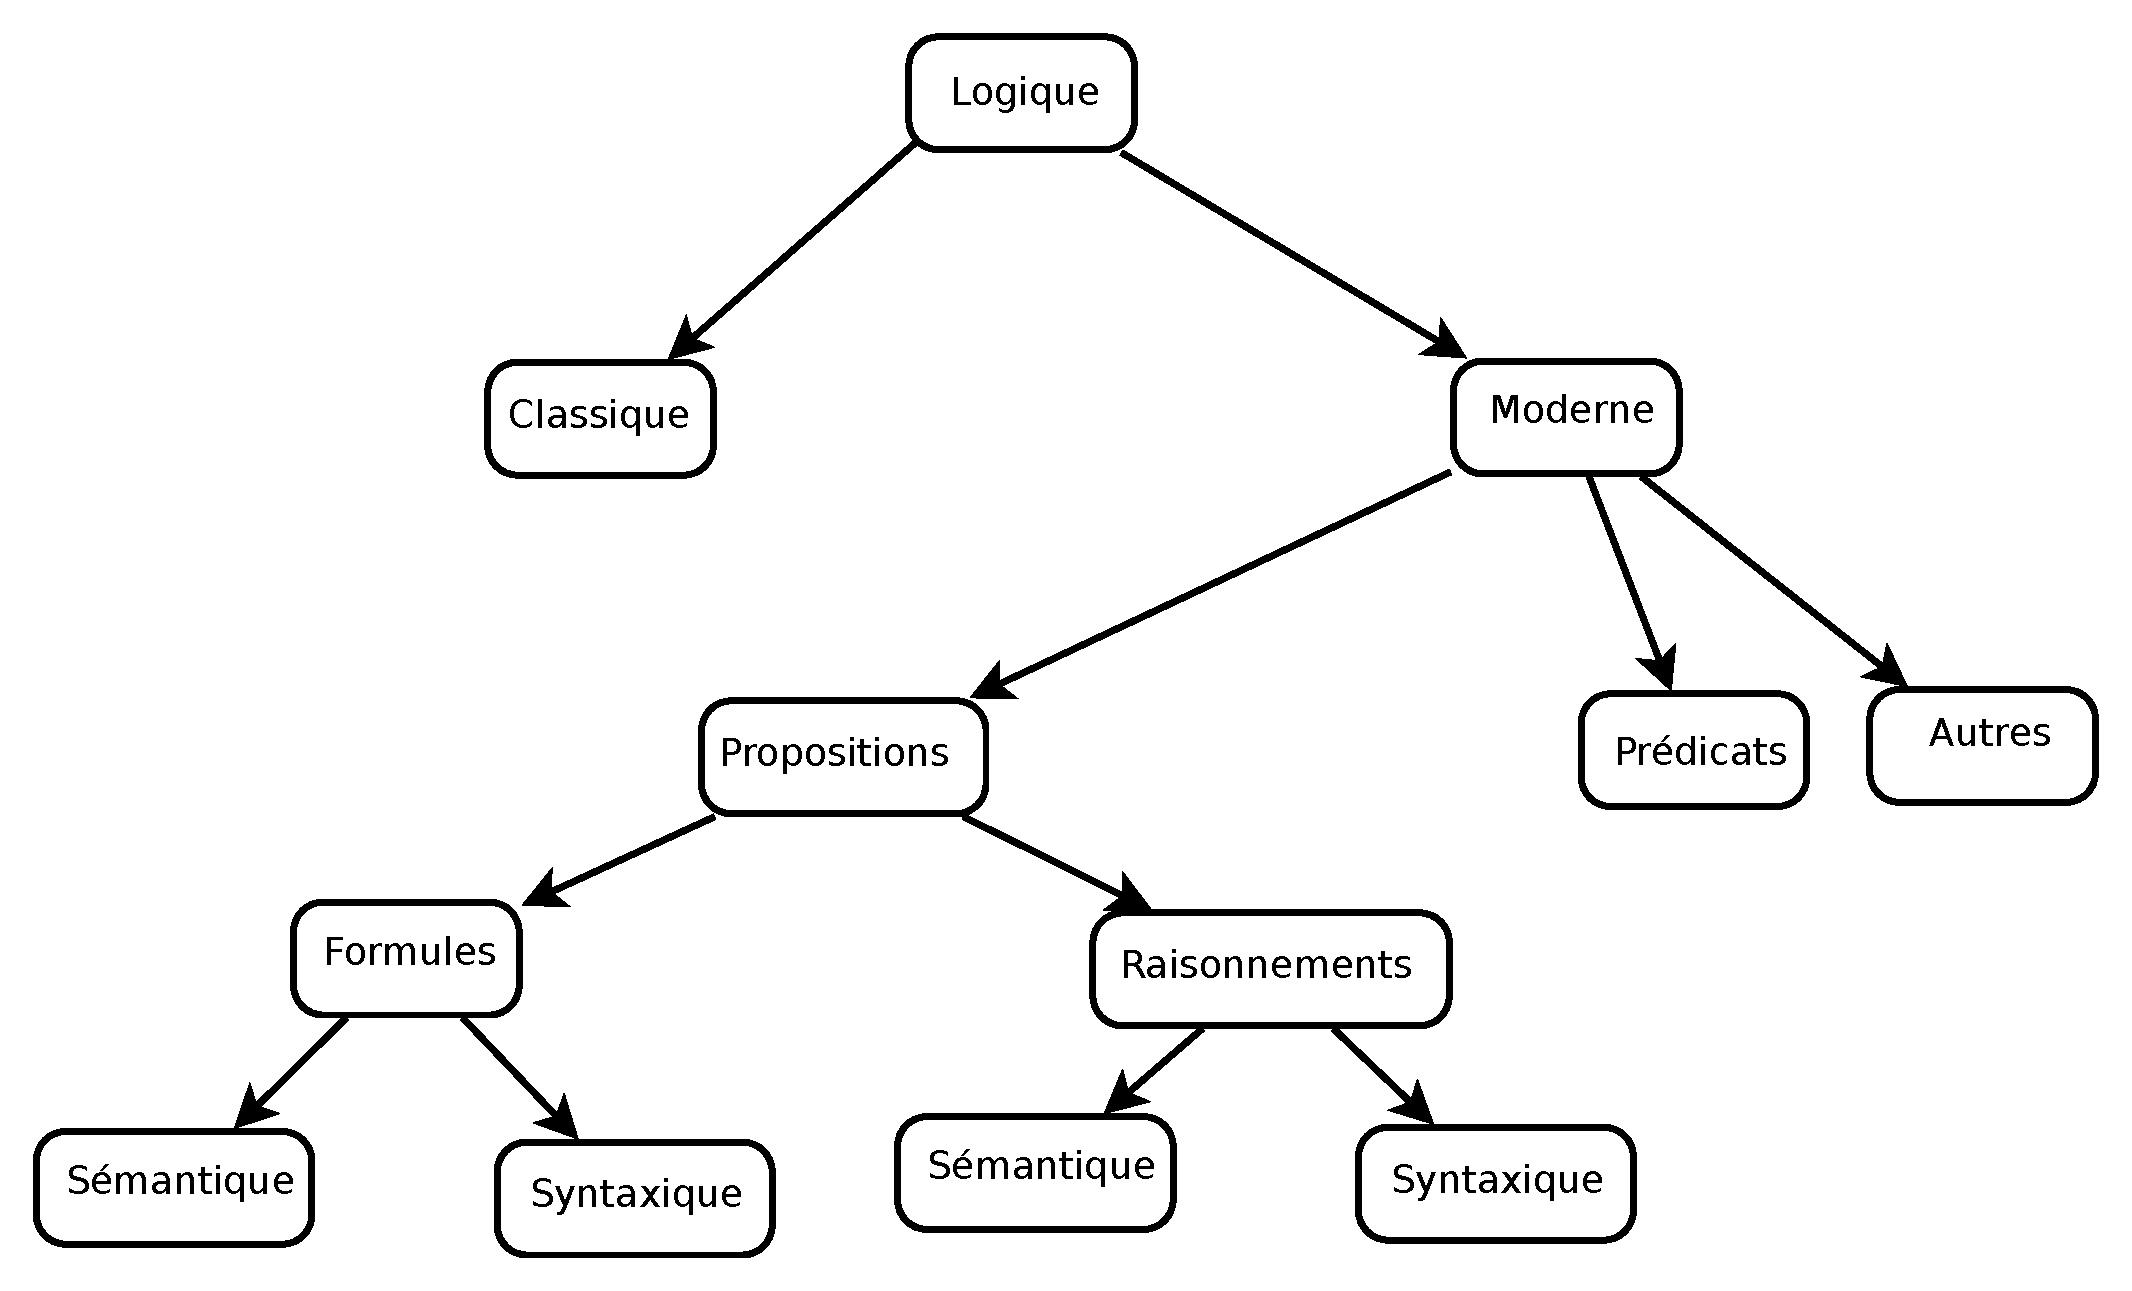
\includegraphics[width=\linewidth]{fig1_types.pdf}\\

\titre{Ordre 0 : Logique des propositions}\\
\titre{Ordre 1 : Logique des prédicats}\\
\titre{Autres :} Logique d'ordre supérieur (quantification des prédicats), logique déviantes (fonctions de vérité à valeurs dans un ensemble de cardinal strictement supérieur à 2)


\fiche{Langage des formules}
\titre{Proposition} : Une proposition ou énoncé ou affirmation est ce qui est vrai ou faux. \\

\titre{Opérateurs} : $\daleth, \vee, \wedge, \rightarrow, \leftrightarrow$\\

\titre{Séparateurs} : $(,),\{,\},[,]$\\

\titre{Formules bien formées (fbf ou wff) }: C'est le plus petit ensemble tel que : 
\begin{itemize}
	\item Toute proposition est une formule (\titre{formule atomique})
	\item Si $A$ et $B$ sont des formules, alors : \\$\daleth A, (A\vee B), (A\wedge B), (A \rightarrow B), (A\leftrightarrow B)$ sont des formules.
\end{itemize}

\titre{Attention} Ne pas confondre langage et méta-langage. \\

\titre{Représentation arborescente} (exemple : $(p\wedge (q\vee r))$ )\\
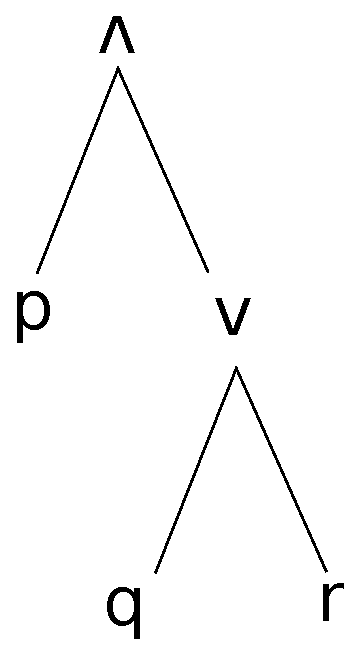
\includegraphics[width=0.15\linewidth]{fig2_arbo.pdf}


\fiche{Sémantique des formules}
\titre{Domaine sémantique} (domaine d'interprétation, domaine de discours) : $\{0,1\}$.
\titre{Interpréter une fbf} consiste à lui attribuer une valeur de $\{0,1\}$\\

\titre{Une assignation} sur $n$ propositions est un ensemble d'interprétations de ces propositions (un $n-$uplet). Une assignation = un monde possible = une ligne de la table de vérité (pour $n$ proposition il y a $2^n$ assignations possibles et $2^{2^n}$ fonctions de vérité possibles). \\

\titre{Un modèle} pour une fbf donnée est une assignation qui la rend vraie. \\

\titre{Méthode} Pour déterminer la sémantique d'une formule, on dresse sa table de vérité. \\

\titre{Théorème de substitution} Si une formule est valide (resp. inconsistante), la formule obtenue en substituant chaque occurence d'un schéma de formule par une fbf quelconque est également valide (resp. inconsistante).\\

\titre{Métalangage} $\conslogiquedble$ A signifie A est valide.




\fiche{Théories syntaxiques}
\titre{Formules de De Morgan} : 
\begin{itemize}
  \item $\non (p \et q) \equi \non p \ou q$
  \item $\non (p \ou q) \equi \non p \et \non q$
\end{itemize}
\titre{Formule sans nom} : $(p\ou q) \rightarrow (p\et q) \equi p \leftrightarrow q$\\
\titre{Equivalence} $A \equi B$ si et seulement si $\conslogiquedble A \leftrightarrow B$ \\



\fiche{Algèbre de Boole}
\titre{Définition} : $(\mathcal{B},\et,\ou,\non)$ où $\mathcal{B} = \{0;1\}$ avec $0$ est la classe d'équivalence de $p\et\non p$ et $1$ est la classe d'équivalence de $p\ou\non p$ pour la relation $\equi$\\

\titre{Propriétés}
\begin{itemize}
  \item Idempotence : $A\et A \equi A; A\ou A \equi A$
  \item Non contradiction : $A\et \non A \equi O$ (symétrique pour $\et$)
  \item Tiers exclu : $A \ou \non A \equi 1$ (symétrique pour $\ou$)
  \item Bivalence : $\non 1 \equi 0$ et $\non O \equi 1$
  \item Double négation : $\non \non A \equi A$
  \item Eléments neutres : $A\et 1 \equi A$ et $A \ou 0 \equi A$
  \item Eléments absorbants : $A \et 0 \equi 0$ et $A \ou 1 \equi 1$
  \item Commutativité de $\et$ et $\ou$
  \item Associativité de $\et$ et $\ou$
  \item Distributivité : $A\et(B\ou C) \equi (A \et B)\ou(A\et C)$ et $A\ou(B\et C) \equi (A\ou B) \et (A \ou C)$
  \item Lois d'absorbtion : $A \ou (A\et B) \equi A$ et $A\et (A\ou B) \equi A$
\end{itemize}

\titre{Equivalences fondamentales}
\begin{itemize}
  \item Loi de De Morgan
  \item $A \leftrightarrow B \equi (A \rightarrow B) \et (B \rightarrow A)$
  \item $A \rightarrow B \equi (\non A \ou B) \equi (\non B \rightarrow \non A)$
\end{itemize}


\fiche{Formes normales}
\titre{Clause} : Est une disjonction de variables propositionnelles éventuellement niées. (suppression des parenthèses à l'intérieur de la clause)\\

\titre{FNC} Une forme normale conjonctive est une conjonction de clauses (utile pour montrer qu'une formule est valide). \\

\titre{FND} Une forme normale disjonctive est une disjonction de conjonctions de variables propositionnelles éventuellement niées (utile pour montrer qu'une formule est inconsistante).\\

\titre{Théorème} Pour toute formule il existe une FND et une FNC équivalentes. (preuve par algorithme) \\

\titre{FND complète} Chaque conjonction contient une et une seule occurence de chaque variable propositionnelle. Pour une formule donnée elle est utile (aux commutations près). 
\\

\titre{Remarque} Les termes de la FND complète correspondent aux modèles de la formule. Valide : $2^n$ termes ; Inconsistante : $0$ termes.


\fiche{Méthode des arbres}
\titre{Règles de réécriture}\\
$\begin{array}{c} A\et B \\ | \\ A \\ B \end{array}$
\hspace{2cm}
$\begin{array}{ccc} & A \ou B & \\  & / \hspace{0.7cm} \backslash & \\ A &  & B \end{array}$
\hspace{2cm}
$\begin{array}{ccc} & \non (A \et B) & \\ & / \hspace{0.7cm} \backslash & \\ \non A & & \non B \end{array}$
\hspace{2cm} \\ \\ \vspace{1cm}
$\begin{array}{c} \non (A\ou B) \\ | \\ \non A \\ \non B \end{array}$
\hspace{2cm}
$\begin{array}{c} \non\non A \\ | \\ A \end{array}$
\hspace{2cm}
$\begin{array}{ccc} & A \rightarrow B & \\ & / \hspace{0.7cm} \backslash & \\ \non A & & \non B \end{array}$
\hspace{2cm}\\ \\ \vspace{1cm}
$\begin{array}{ccc} & A \leftrightarrow B & \\ & / \hspace{0.7cm} \backslash & \\ \non A & & A \\ \non B & & B \end{array}$
\hspace{2cm}
$\begin{array}{c} \non (A \rightarrow B) \\ | \\ A \\ \non B \end{array}$
\hspace{2cm} \\ \\ \vspace{1cm}
$\begin{array}{ccc} & \non (A \leftrightarrow B) & \\ & / \hspace{0.7cm} \backslash & \\ A & & \non A \\ \non B & & B \end{array}$\\

\titre{Méthode}
\begin{itemize}
  \item On ferme un chemin dès qu'il contient une formule et sa négation. 
  \item Les chemins non fermés donnent un terme de la FND
  \item Si tous les chemins sont fermés, c'est une contradiction
\end{itemize}


\end{document}
